\chapter{Analyse}

\begin{itemize}
  \item Daten
  \begin{itemize}
    \item Welche Listen wurden verwendet?
    \item Woher kommen die?
  \end{itemize}
  \item Statistische Auswertung
  \begin{itemize}
    \item Gesamtauswetungen
    \item Kleine Abschnitte für Einzelauswertungen der Tests
  \end{itemize}
  \item Disskusion
  \item Bewertung
\end{itemize}
\todo{Samuel}

Nachdem die Seiten von webifier überprüft und in der Datenbank abgelegt worden sind werden sie von webifier-statistics für die Auswertung genutzt. Hier wird eine interaktive Weboberfläche erzeugt. Abbildung \ref{fig:dashboard} zeigt den Einstiegspunkt auf die Webseite. Hier sind Zahlen über die Anzahl der getesteten Seiten pro Tag und insgesamt aufgelistet. Diese werden anhand des Ergebnisses gruppiert. Zusätzlich findet sich hier noch die durchschnittliche Analysezeit für eine Webseite. Darunter ist eine Beschreibung was webifier-statistics ist.

Die Grafik visualisiert die Aktivität von webifier über den gesamten, von webifier-data, gespeicherten Zeitraum. Die Schwankungen in der Analyseaktivität sind zum einen auf 2 Serverausfälle zurückzuführen. Des Weiteren gibt es Abweichungen, da die Analysezeit abhängig von der Größe und Komplexität der Webseite ist. So wurden an Tagen mit weniger Aktivität komplexere Webseiten getestet.
\begin{figure}[H]
  \centering
  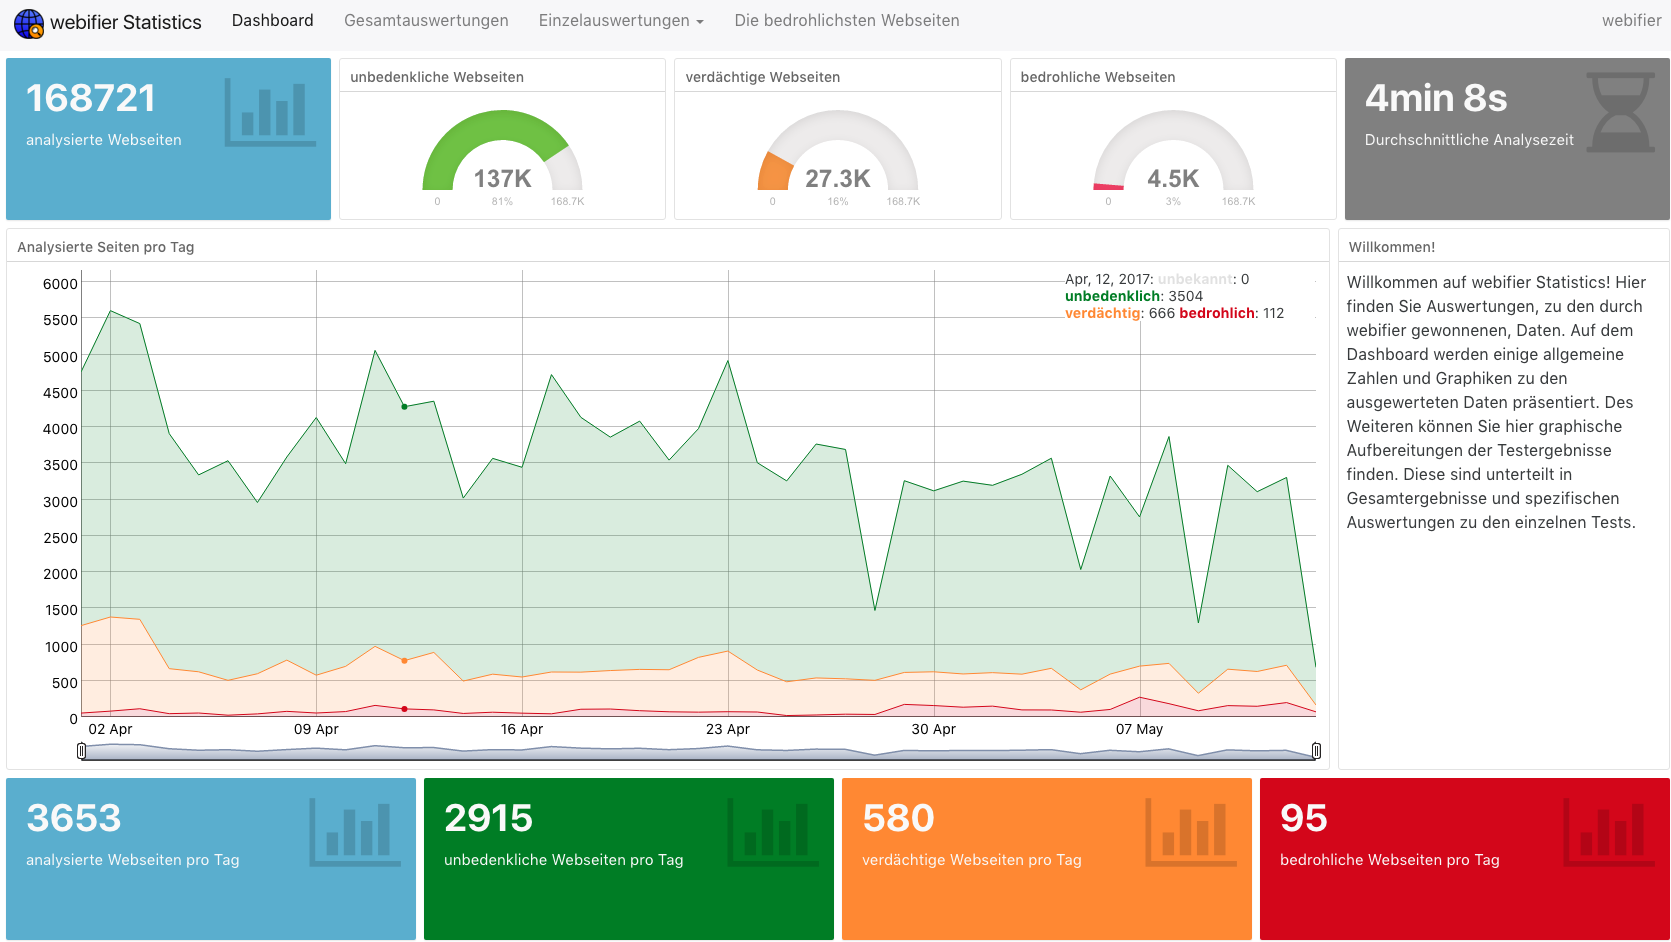
\includegraphics[width=15cm]{images/stats/dashboard}
  \caption{Webifier Statistics Dashboard}
  \label{fig:dashboard}
\end{figure}

An der Oberkante ist eine Navigationsleiste zu finden. Diese wird auf allen Teilseiten angezeigt. Der Nutzer kann hier zwischen den einzelnen Seiten wechseln, hinter dem Reiter \textit{Einzelauswertungen} befindet sich ein Dropdown-Menü zur Auswahl des jeweiligen Testes für den der Nutzer die Statistiken betrachten möchte. In den nachfolgenden Kapiteln wird auf diese Auswertungen genauer eingegangen.

\section{Gesamtauswertungen}
In den Gesamtauswertungen finden sich alle Statistiken, die sich auf die Gesamttests der Webseite beziehen. Ein Gesamttest ist der komplette Durchlauf aller Tests einer Webseite mit aggregiertem Ergebnis. In den folgenden Abschnitten werden die Grafiken beschrieben, die dort zu finden sind.

Der Nutzer hat hier wieder die Möglichkeit über eine zweite Navigationsleiste zwischen den einzelnen Statistiken zu wechseln(siehe Abbildung \ref{fig:tlderkennungen} oben). In den folgenden Abbildungen wird dies zugunsten der Übersichtlichkeit nicht angezeigt.

Die erste Statistik(Abbildung \ref{fig:tlderkennungen}) visualisiert die Anzahl der bedrohlichen und verdächtigen Funde anhand der \ac{TLD}. Zur besseren Übersichtlichkeit werden hier nur Seiten mit bedrohlichem oder verdächtigem Ergebnis gezeigt. Diese werden dann anhand ihrer \ac{TLD} aggregiert und als Balkendiagramm dargestellt. Es werden nur \ac{TLD}, welche mindestens 50 Einträge in der Datenbank haben. Der rote Balken steht für die Anzahl an bedrohlichen Ergebnissen der jeweiligen \ac{TLD} und der gelbe Balken für die verdächtigen Funde. Es fällt auf, dass die \ac{TLD} .com und .de die größten Anteile an beiden Balken haben. Dies ist darauf zurückzuführen, dass diese im \ac{WWW} am weitesten verbreitet sind. Da hier nicht die prozentuale Verteilung der Ergebnisse auf eine \ac{TLD} zu erkennen ist, kann nur Aussage über die Anzahl der Funde in der Datenbank Aussage getroffen werden. Die allgemeine Bedrohlichkeit einer \ac{TLD} kann hieraus nicht abgeleitet werden.
\begin{figure}[H]
  \centering
  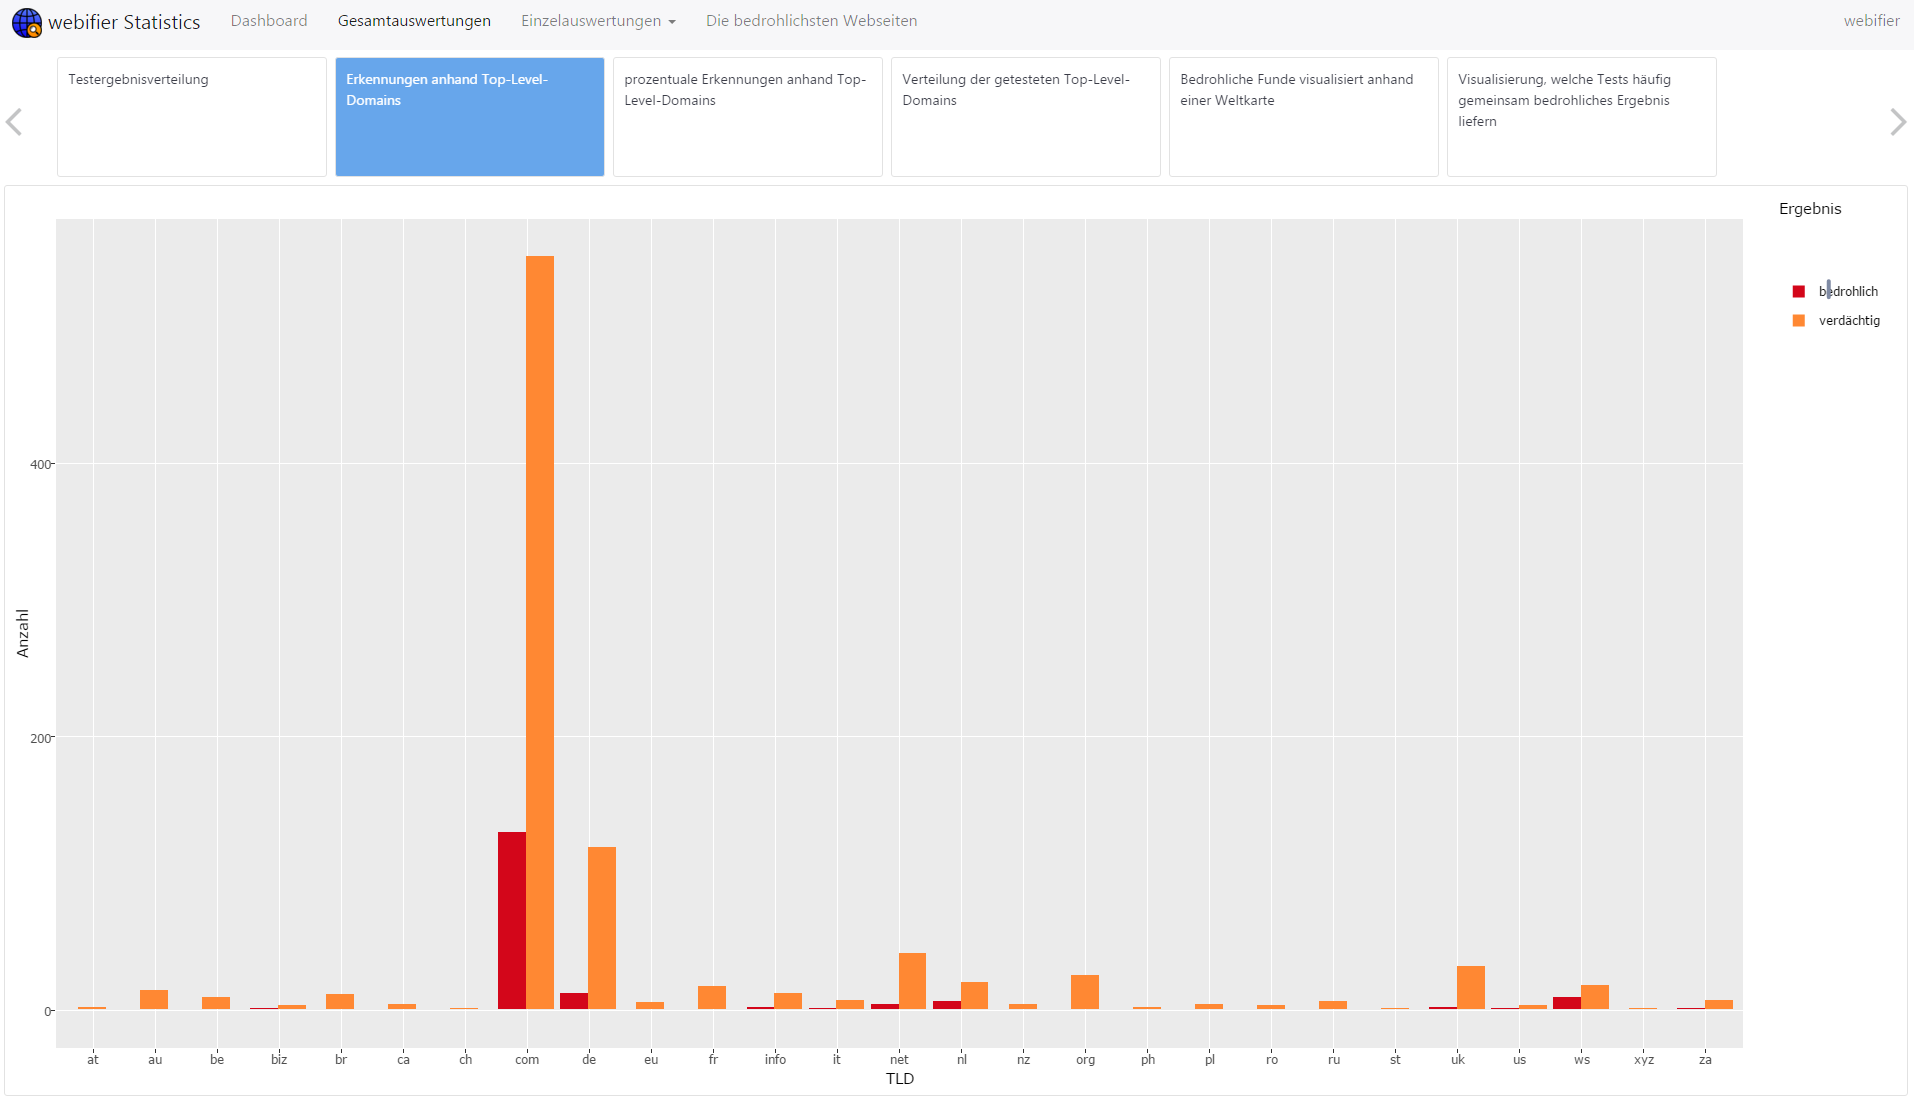
\includegraphics[width=15cm]{images/stats/tlderkennungen}
  \caption{Erkennungen anhand Top-Level-Domains}
  \label{fig:tlderkennungen}
\end{figure}

Das, in Abbildung \ref{fig:tldverteilung} dargestellte, Tortdendiagramm zeigt die Verteilung der getesteten Ergebnisse anhand der \ac{TLD} auf. Auch hier bilden die Top-Level Domains .com (blau - 57.1\%) und .de (orange - 12.5\%) den größten Anteil. Dies bestätigt den Inhalt der vorherigen Grafik, dass diese \ac{TLD},auch für maliziöse Zwecke, sehr verbreitet sind. Sie werden gefolgt von ebenfalls bekannten Adressen wie .net oder .uk.
\begin{figure}[H]
  \centering
  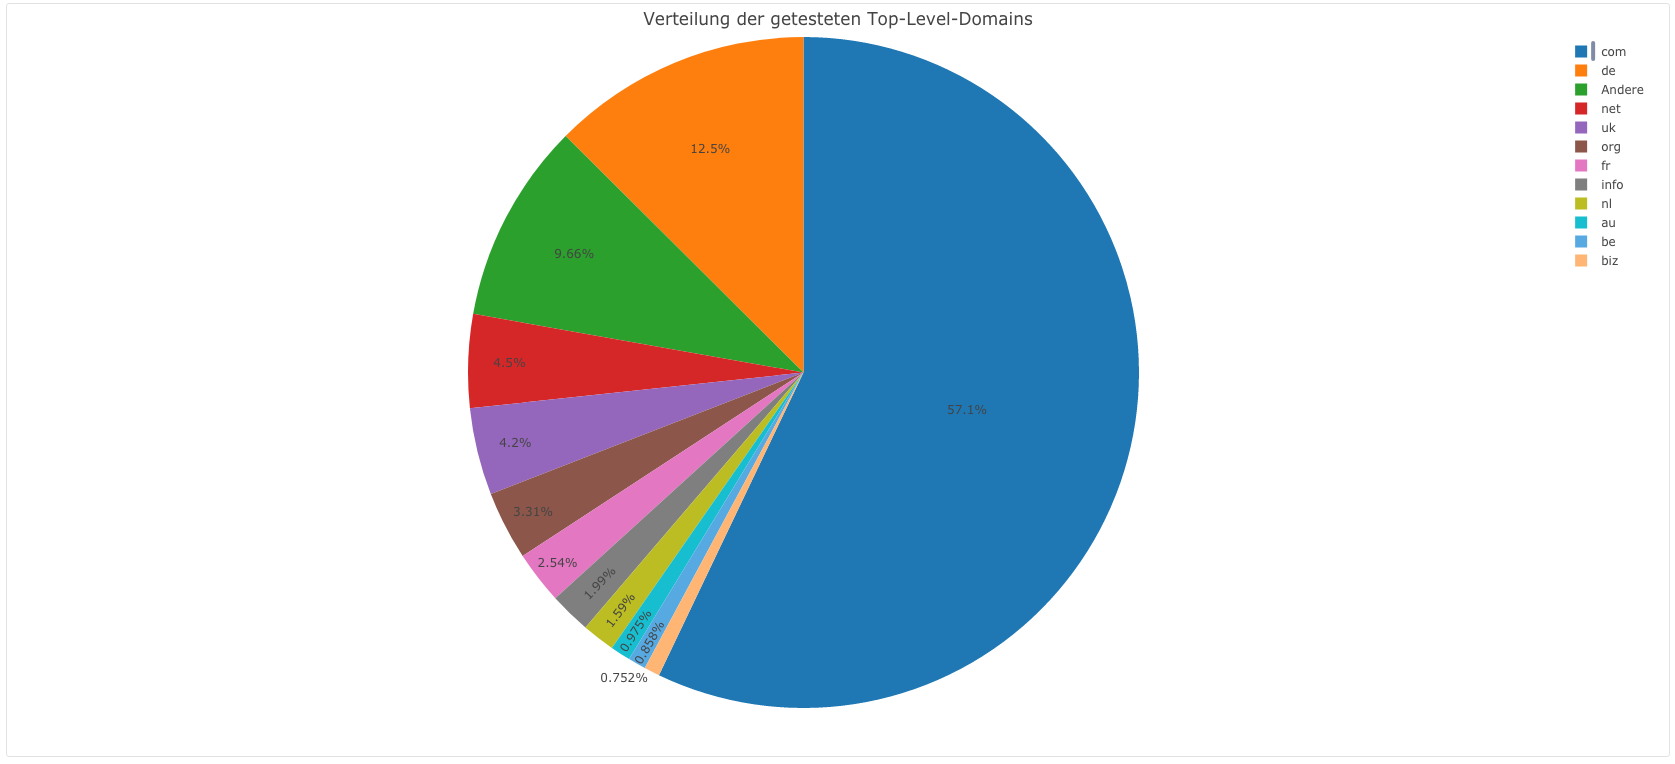
\includegraphics[width=15cm]{images/stats/tldverteilung}
  \caption{Verteilung der getesteten Top-Level-Domains}
  \label{fig:tldverteilung}
\end{figure}

Die Abbildung \ref{fig:tldprozentual} befasst sich ebenfalls mit den Top-Level Domains. Hier wird die prozentuale Verteilung der Ergebnisse unbedenklich(grün),verdächtig(gelb) und bedrohlich(rot) aufgezeigt. Hier fällt auf, dass die bedrohlichsten \ac{TLD}s eher unbekannte sind, wie beispielsweise .pictet oder .sa. Diese beiden kommen auf jeweils 100\% bedrohliche Ergebnisse. Das bedeutet, dass jede Seite mit dieser \ac{TLD} von webifier als bedrohlich erkannt wurde. Die .com-Domain liegt hier im Mittelfeld mit knappen 80\% sauberen Webseiten. Weiterhin ist zu sehen, dass die deutsche \ac{TLD}(.de) in der Liste nicht auftaucht. Dies ist darauf zurückzuführen, dass für diese Auswertung alle Top-Level-Domains mit 100\% sauberen Webseiten vernachlässigt wurden. Wie aus Abbildung \ref{fig:tlderkennungen} bekannt, wurden aber auch hier bedrohliche Seiten gefunden. Diese sind prozentual gesehen jedoch ein so geringer Anteil, dass sie durch Rundung vernachlässigt wurden.
\begin{figure}[H]
  \centering
  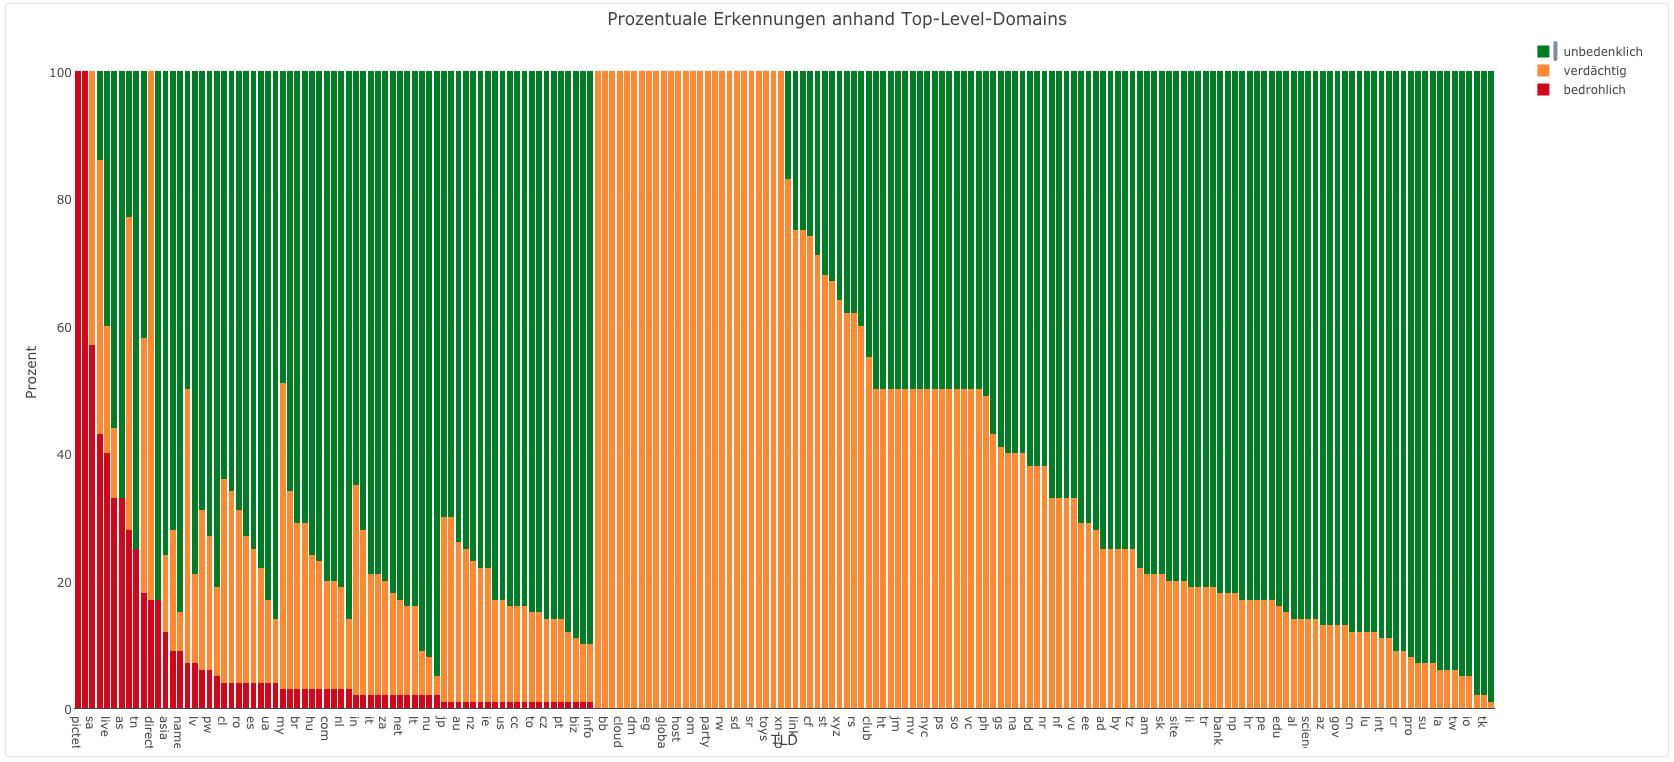
\includegraphics[width=15cm]{images/stats/tldprozentual}
  \caption{prozentuale Erkennungen anhand Top-Level-Domains}
  \label{fig:tldprozentual}
\end{figure}

Aus den 3 Grafiken zur Verteilung bezogen auf die Top-Level Domains kann erkannt werden, dass bestimmte, eher unbekannte, Top-Level Domains öfter für bedrohliche Zwecke verwendet werden. Jedoch werden auch die bekannten (bspw. .com und .de) Adressen genutzt. Dies lässt sich erklären, dass viele Nutzer im \ac{WWW} bei Webseiten, die auf .de oder .com enden unvorsichtig werden und sich sicher fühlen, da ihnen die \ac{TLD} bekannt ist.

In Abbildung \ref{fig:weltkarte} wird eine Weltkarte dargestellt, welche sich anhand des Risikofaktors der Länder verfärbt. Der Risikofaktor berechnet sich aus dem durchschnittlichen Ergebniswert aller Ergebnisse des Landes und dies wird mit 100 multipliziert um den prozentualen Wert zu erhalten. Hierbei werden die \ac{TLD} den Ländern zugeordnet. Domains wie .com, welche nicht auf ein bestimmtes Land zurückgeführt werden können, werden in dieser Auswertung vernachlässigt. Länder, für die es keine Zuordnung gab bleiben unausgefüllt.

Es ist zu schnell zu Erkennen, dass die Top-Level Domains für Saudi Arabien(.sau) und Libyen(.lby) den größten Risikofaktor haben. Ein Problem bei dieser Darstellung ist, dass nur die Top-Level Domain der Internetadresse entscheidend ist für die Zuordnung. Für eine genauere Zuordnung müsste man die Lokation anhand der IP-Adresse herausfinden und diese dann den Ländern zuordnen. Denn eine .sau-Domain bedeutet nicht zwangsläufig, dass der Betreiber der Webseite auch in dem jeweiligen Land ansässig ist. Oft wird die Webseite von einem anderen Standort aus betrieben. Einige Betreiber nutzen eine bestimmte Top-Level Domain auch wegen dem Namen. Des Weiteren könnten mit einer Adressierung über IP-Adresse auch jene \ac{TLD} mit einbezogen werden, welche keinem Land zugeordnet sind.

\begin{figure}[H]
  \centering
  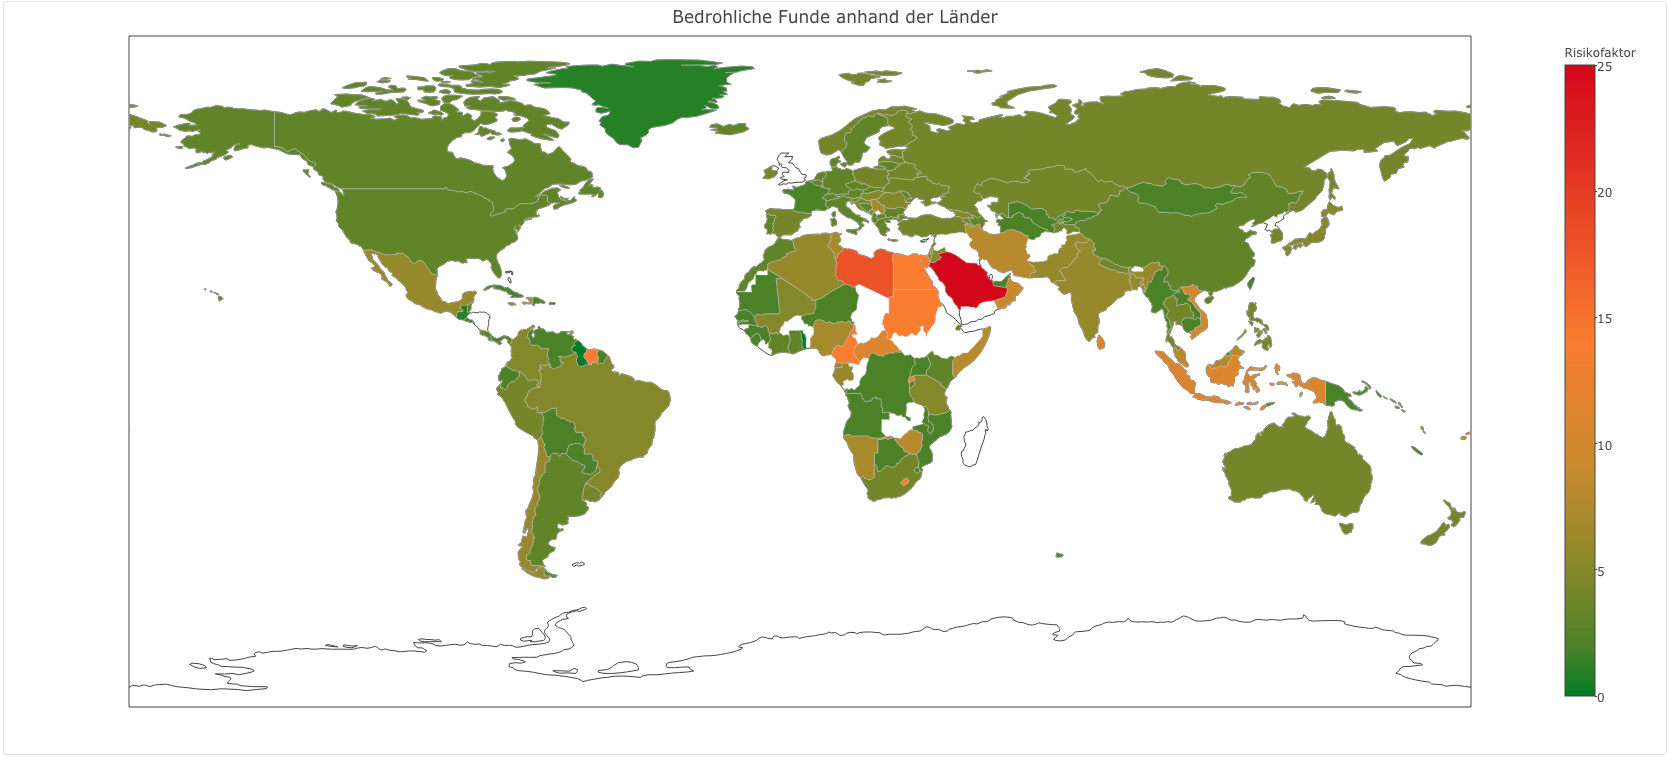
\includegraphics[width=15cm]{images/stats/weltkarte}
  \caption{Bedrohliche Funde visualisiert anhand einer Weltkarte}
  \label{fig:weltkarte}
\end{figure}

Im folgenden Balkendiagramm (siehe Abbildung \ref{fig:ergebnisverteilung}) wird die Verteilung der Ergebnisse der einzelnen Tests dargestellt. Für jeden Test werden bis zu 4 Balken für die jeweiligen Ergebnistypen dargestellt.

Hier fällt auf, dass der IP-Scan-Test und der Virusscan-Test nahezu nur saubere Ergebnisse haben. Desweiteren ist zu Erkennen, dass der CertifikateChecker sehr viele verdächtige Seiten gefunden hat. Was dieser Wert aussagt wird im späteren Kapitel über den Test genauer beleuchtet. Eine weitere Beobachtung gibt es bei dem LinkChecker-Test. Dieser hat viele unbekannte Ergebnisse. Dies ist darauf zurückzuführen, dass gerade zu Anfang der Analyse der Datenbestand sehr gering war, so war die Wahrscheinlichkeit, dass eine verlinkte Seite bereits in unseren Daten vorhanden ist sehr gering, somit hat der LinkChecker oft keine Aussage über die Bedrohlichkeit der Seite treffen können.
\begin{figure}[H]
  \centering
  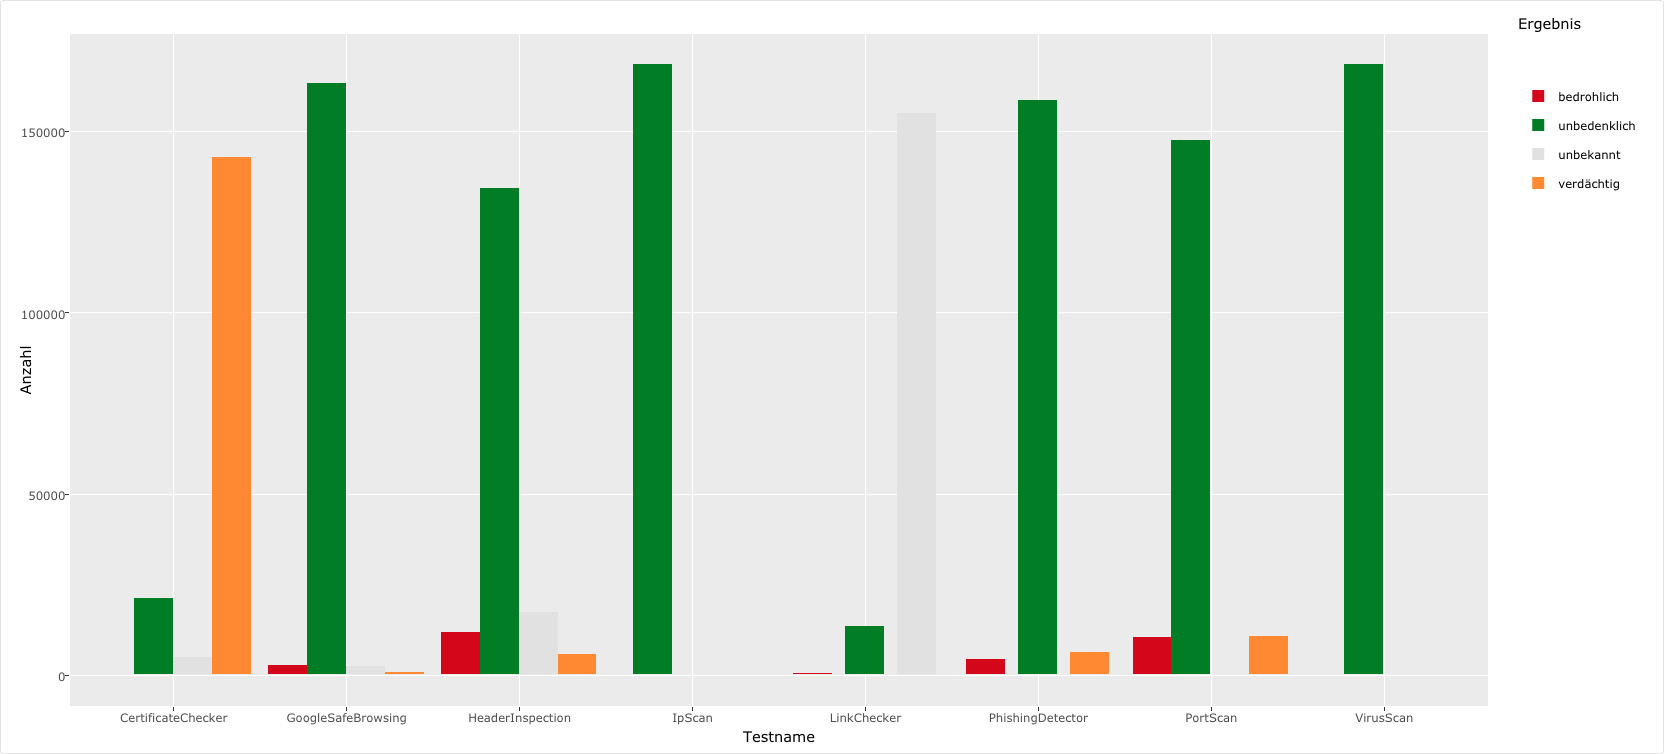
\includegraphics[width=15cm]{images/stats/ergebnisverteilung}
  \caption{Testergebnisverteilung}
  \label{fig:ergebnisverteilung}
\end{figure}

Die nächste Grafik (siehe Abbildung \ref{fig:testzusammenhaenge}) visualisiert die Zusammenhänge der Tests. Es wird aufgezeigt, welche Tests häufig gemeinsam mit anderen Tests das Ergebnis bedrohlich zur gleichen Webseite liefern. Die Größe der einzelnen Punkte wird über die Anzahl der involvierten Tests bestimmt. Die Anzahl sagt aus wie oft diese Tests die gleiche Seite als bedrohlich klassifiziert haben.

Es ist festzustellen, dass am häufigsten die Tests HeaderInspection und PortScan in der Analyse übereinstimmen. Jedoch lässt eine Anzahl von 1.044 Übereinstimmungen bei knapp 170.000 getesteten und ungefährt 4.500 bedrohlichen Seiten nicht auf einen direkten Zusammenhang schließen. Die weiteren Tests schlagen wenig gemeinsam aus, woraus sich kein Zusammenhang feststellen lässt.

\begin{figure}[H]
  \centering
  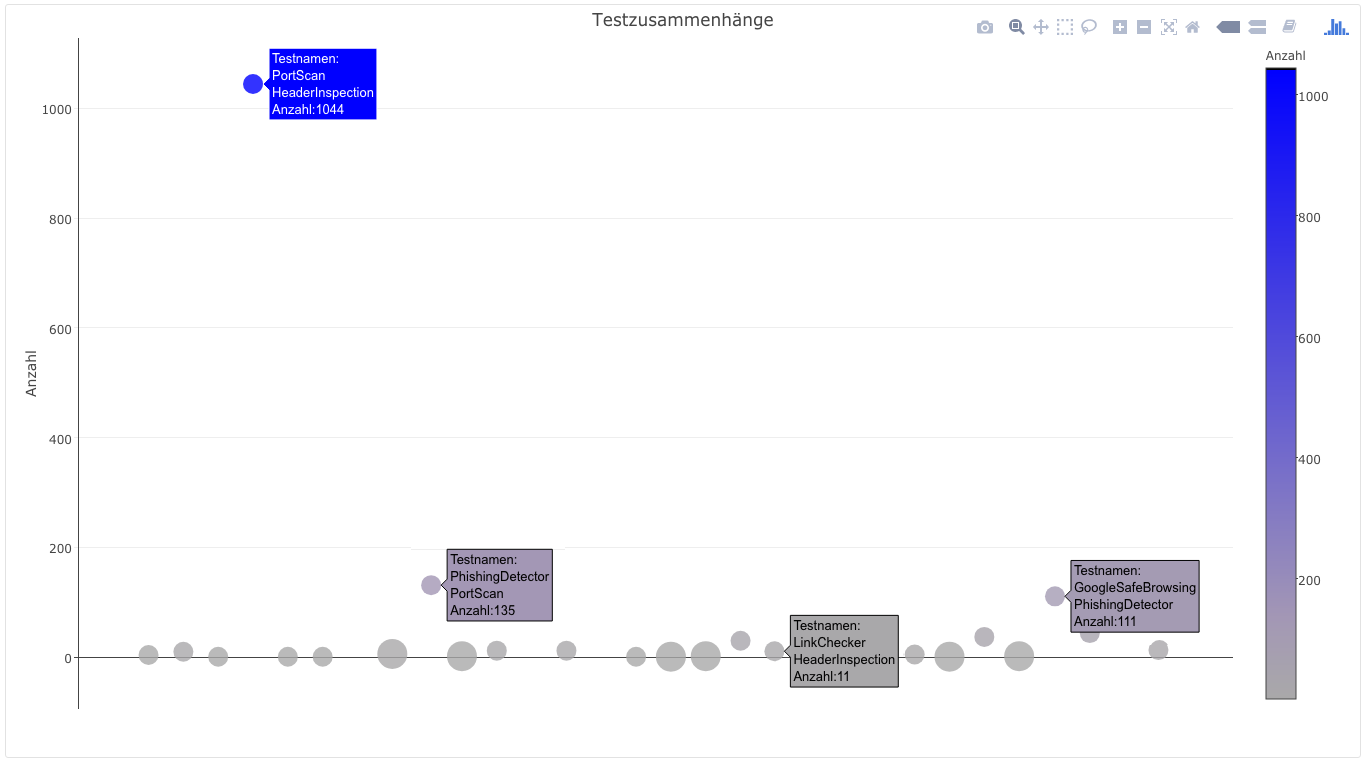
\includegraphics[width=15cm]{images/stats/testzusammenhaenge}
  \caption{Visualisierung der Testzusammenhänge}
  \label{fig:testzusammenhaenge}
\end{figure}

Die Tabelle in Abbildung \ref{fig:top10} gehört nichtmehr direkt zu den Gesamtauswertungen. Sie ist unter einem eigenen Reiter angesiedelt und dient dazu dem Nutzer zu zeigen, welche Seiten den größten Ergebniswert hatten.
\begin{figure}[H]
  \centering
  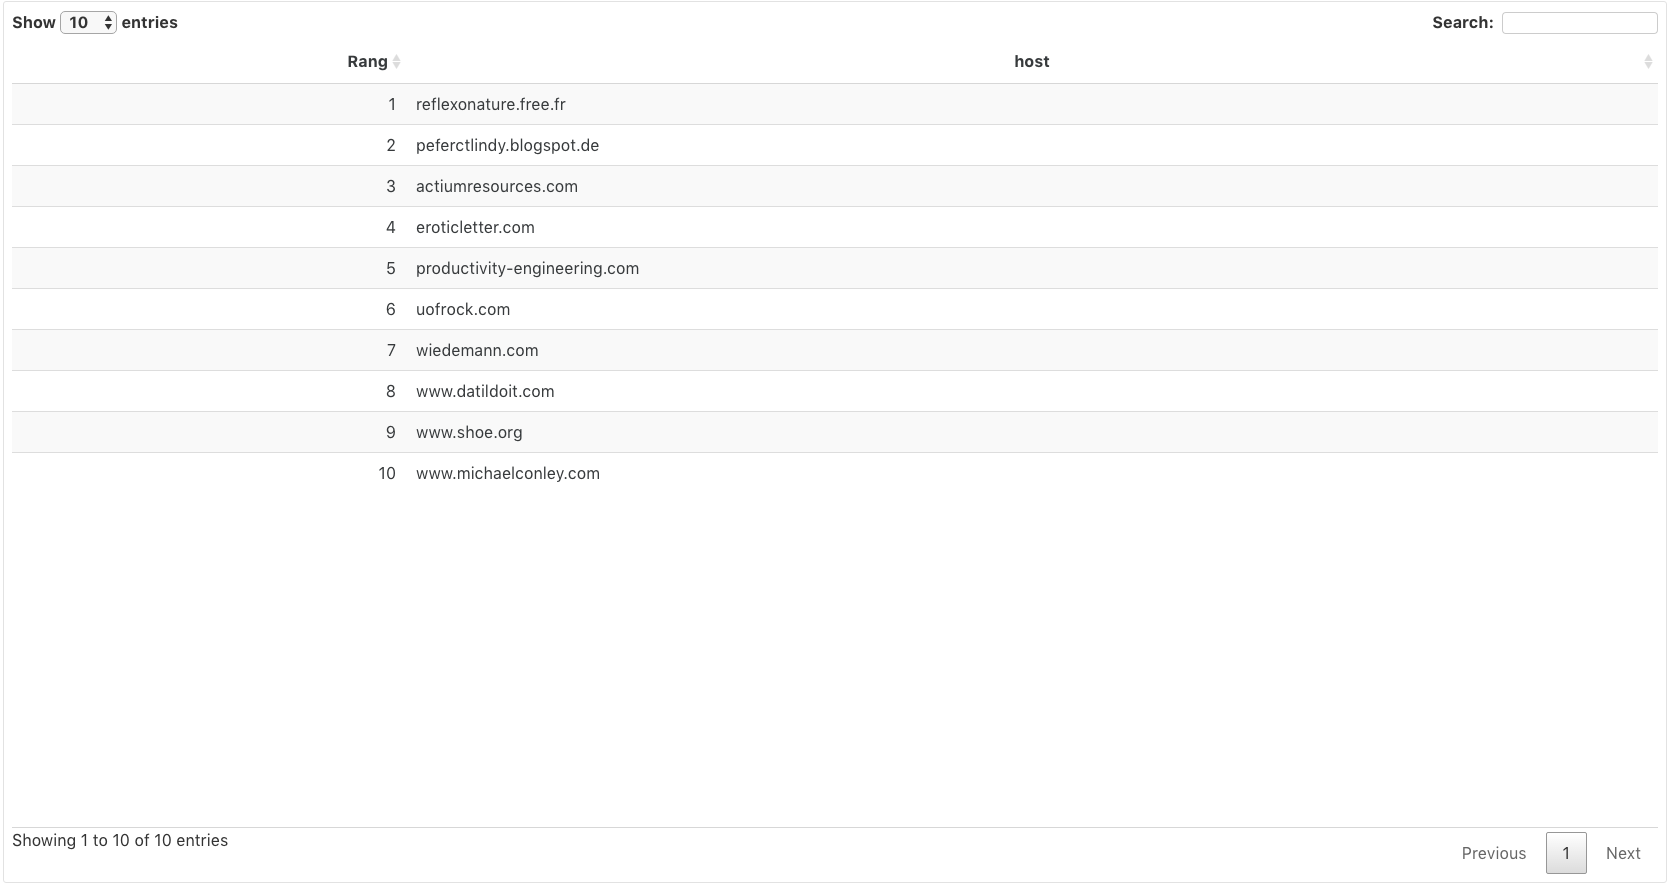
\includegraphics[width=15cm]{images/stats/top10}
  \caption{Top 10: Die bedrohlichsten Webseiten}
  \label{fig:top10}
\end{figure}


\section{Einzelauswertungen}
\begin{figure}[H]
  \centering
  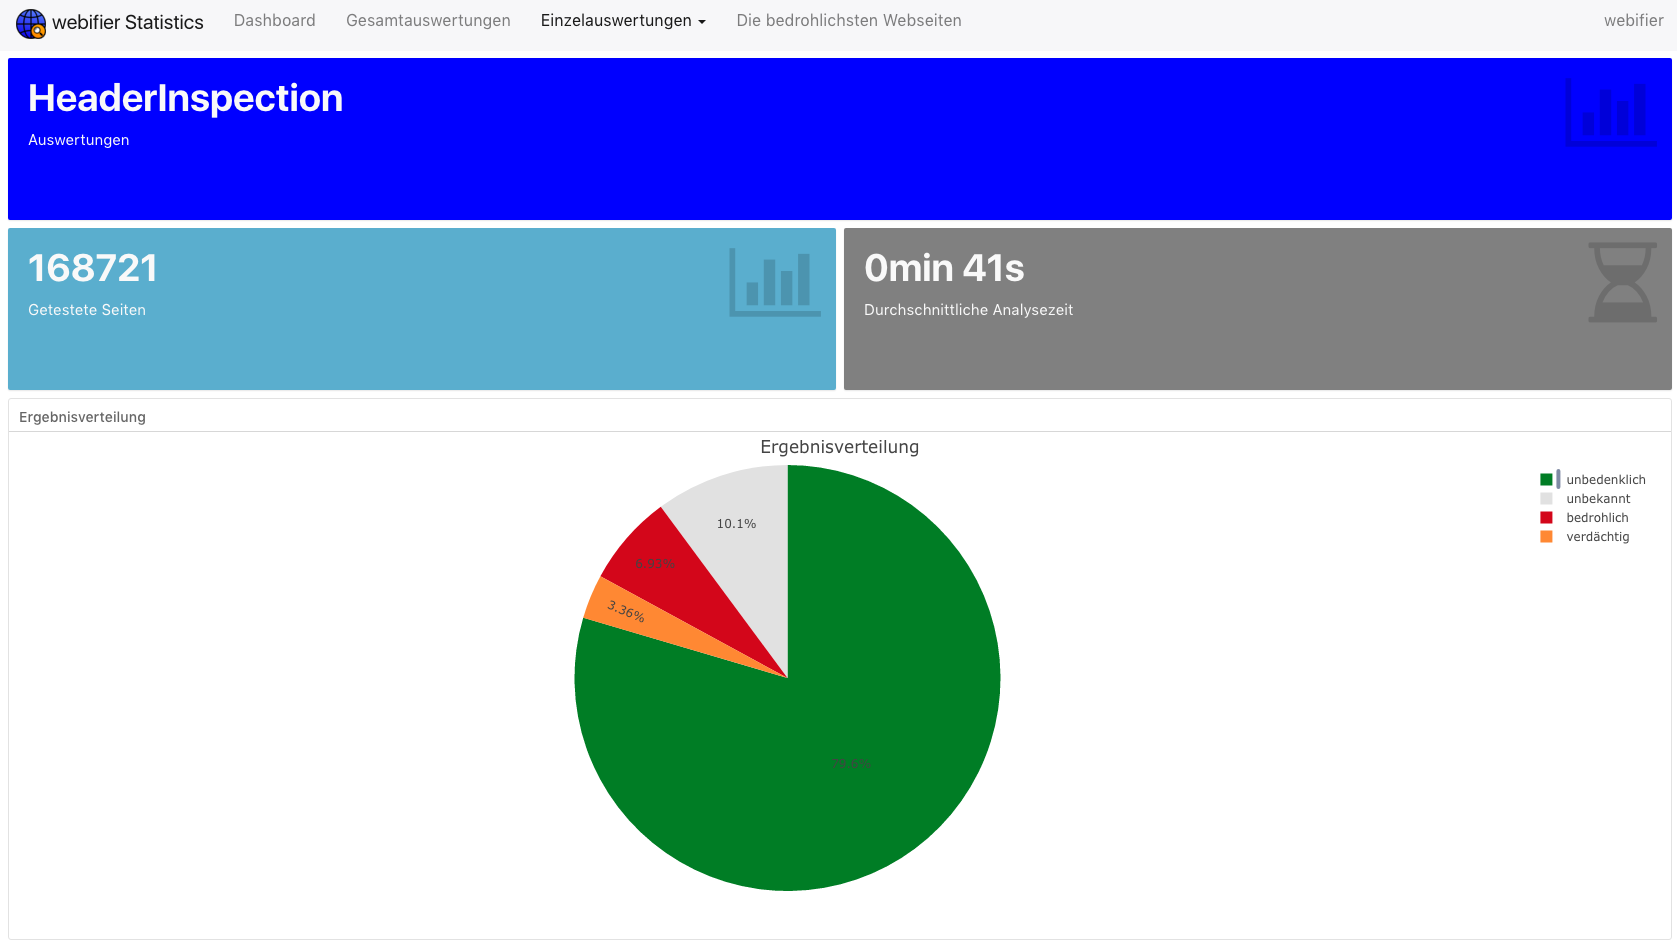
\includegraphics[width=15cm]{images/stats/headerinspection}
  \caption{Einzelauswertung: Vergleich in verschiedenen Browsern}
  \label{fig:headerinspection}
\end{figure}


\begin{figure}[H]
  \centering
  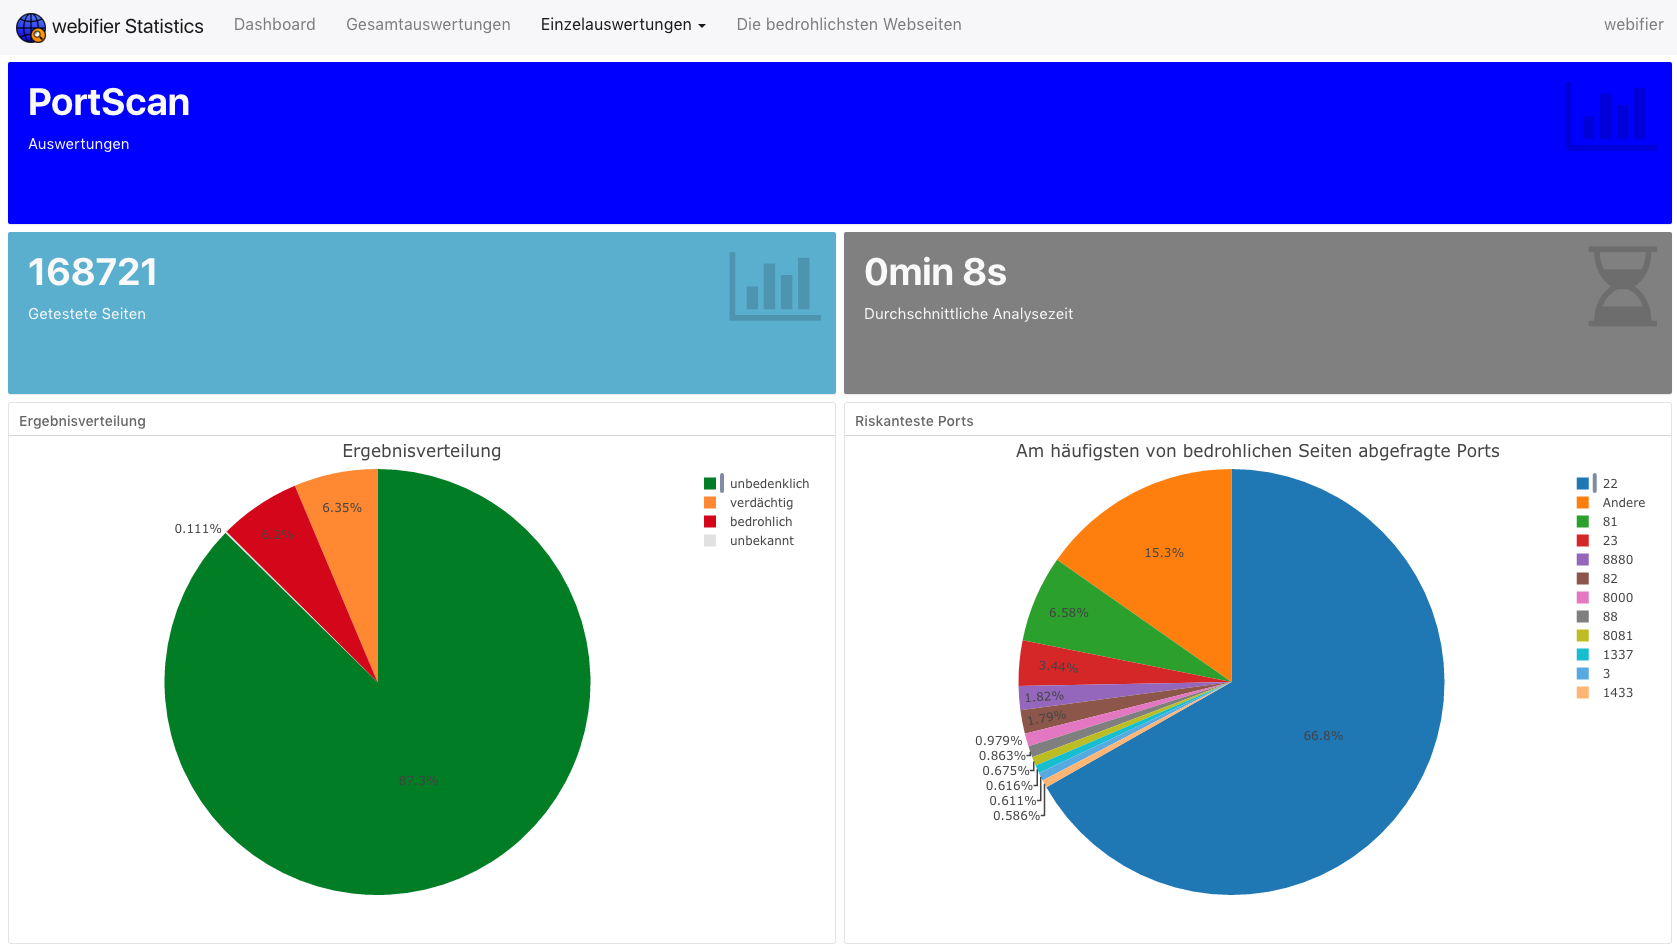
\includegraphics[width=15cm]{images/stats/portscan}
  \caption{Einzelauswertung: Überprüfung der Port-Nutzung}
  \label{fig:virenscan}
\end{figure}


\begin{figure}[H]
  \centering
  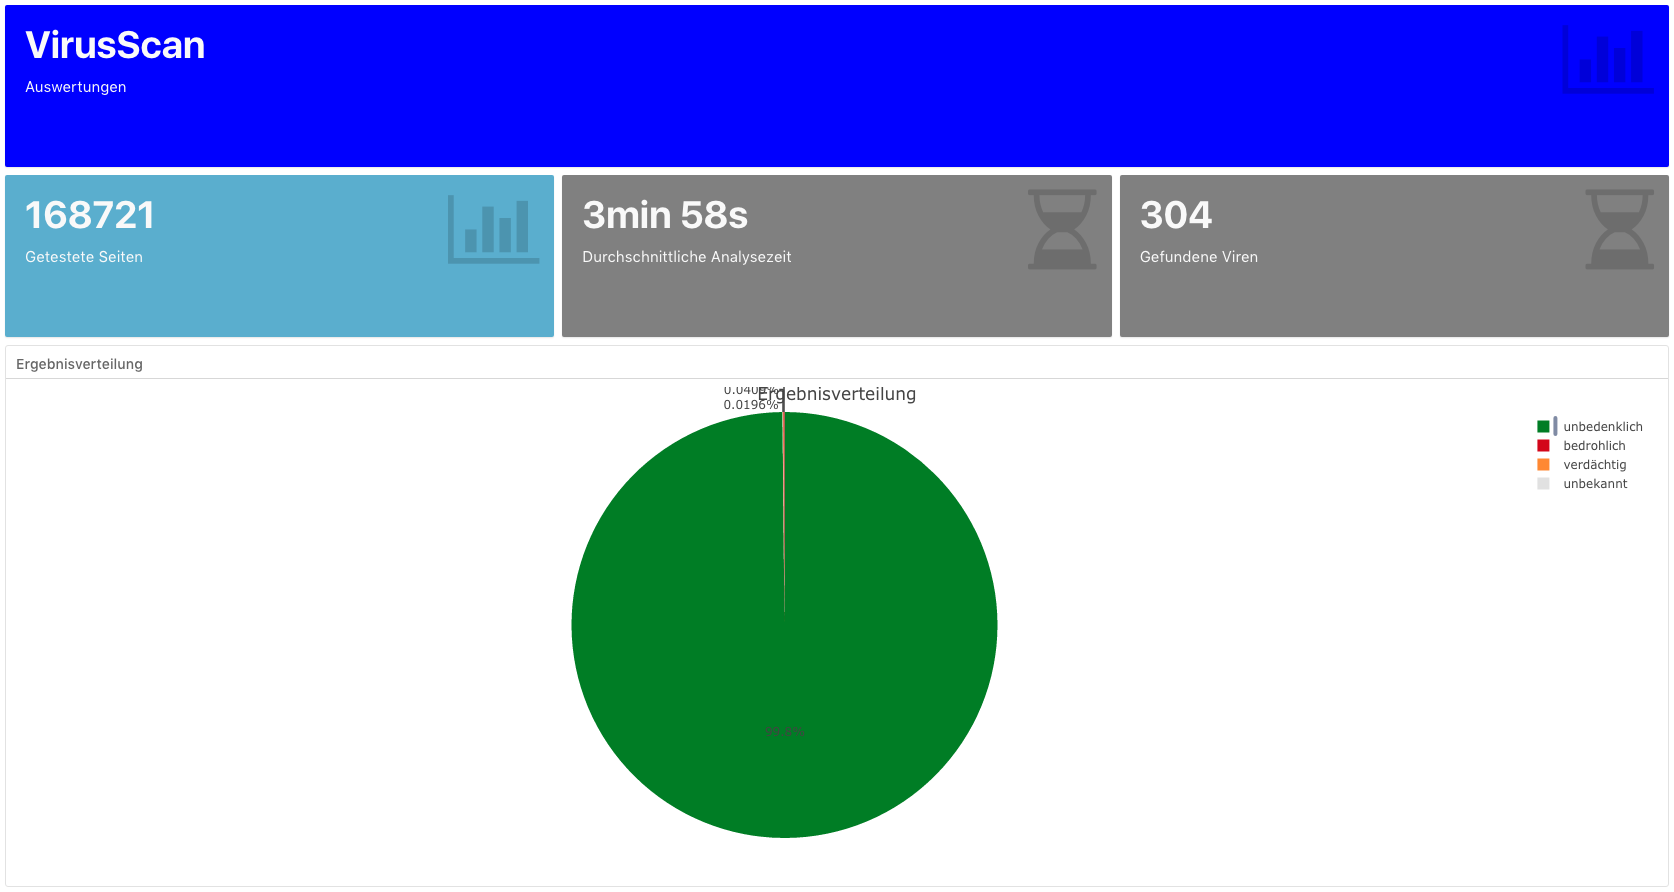
\includegraphics[width=15cm]{images/stats/virusscan}
  \caption{Einzelauswertung: Virenscan der Webseite}
  \label{fig:virusscan}
\end{figure}

\todo{Jani}


\subsection{Virenscan der Webseite}
\begin{figure}[H]
  \centering
  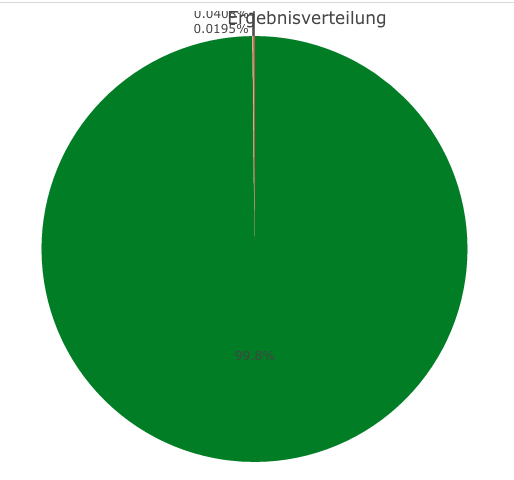
\includegraphics[width=5cm]{images/stats/diavirenscan}
  \caption{Virenscan der Webseite - Testergebnisverteilung}
  \label{fig:diavirenscan}
\end{figure}
\todo{Samuel}

\subsection{Vergleich in verschiedenen Browsern}
\begin{figure}[H]
  \centering
  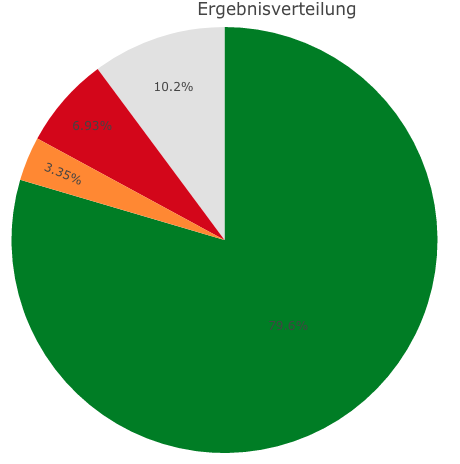
\includegraphics[width=5cm]{images/stats/diaheaderinspection}
  \caption{Vergleich in verschiedenen Browsern - Testergebnisverteilung}
  \label{fig:diaheaderinspection}
\end{figure}
\todo{Daniel}

\subsection{Überprüfung der Port-Nutzung}
\begin{figure}[H]
  \centering
  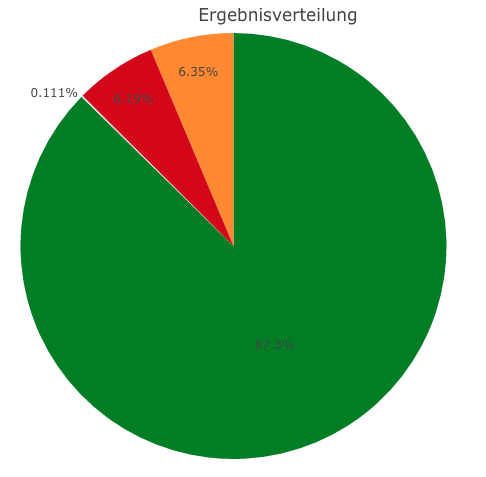
\includegraphics[width=5cm]{images/stats/diaportscan}
  \caption{Überprüfung der Port-Nutzung - Testergebnisverteilung}
  \label{fig:diaportscan}
\end{figure}
\todo{Jani}

\subsection{Überprüfung der IP-Nutzung}
\begin{figure}[H]
  \centering
  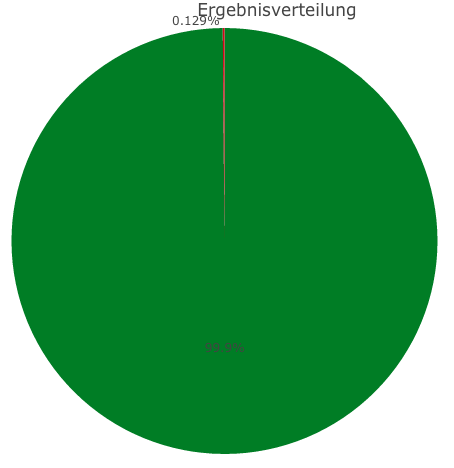
\includegraphics[width=5cm]{images/stats/diaipscan}
  \caption{Überprüfung der IP-Nutzung - Testergebnisverteilung}
  \label{fig:diaipscan}
\end{figure}
\todo{Jani}

\subsection{Prüfung aller verlinkten Seiten}
\begin{figure}[H]
  \centering
  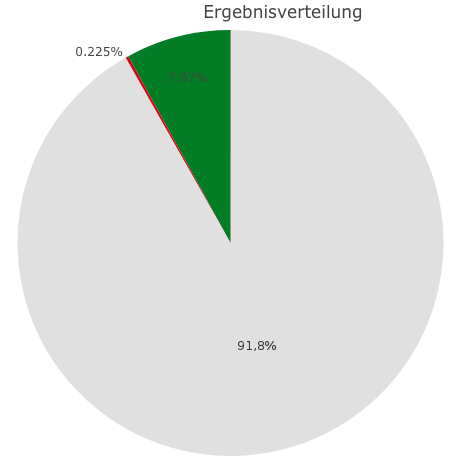
\includegraphics[width=5cm]{images/stats/dialinkchecker}
  \caption{Prüfung aller verlinkten Seiten - Testergebnisverteilung}
  \label{fig:dialinkchecker}
\end{figure}
\todo{Samuel}

\subsection{Google Safe Browsing}
\begin{figure}[H]
  \centering
  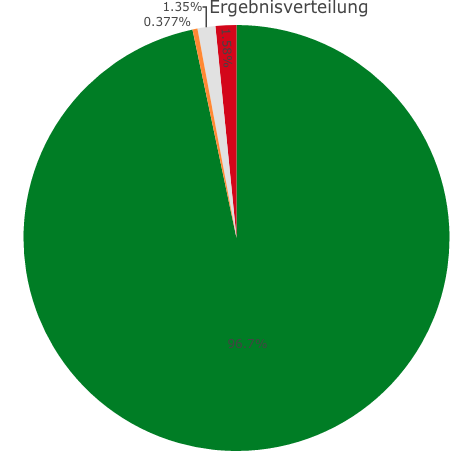
\includegraphics[width=5cm]{images/stats/diagoogle}
  \caption{Google Safe Browsing - Testergebnisverteilung}
  \label{fig:diagoogle}
\end{figure}
\todo{Daniel}

\subsection{Überprüfung des SSL-Zertifikats}
\begin{figure}[H]
  \centering
  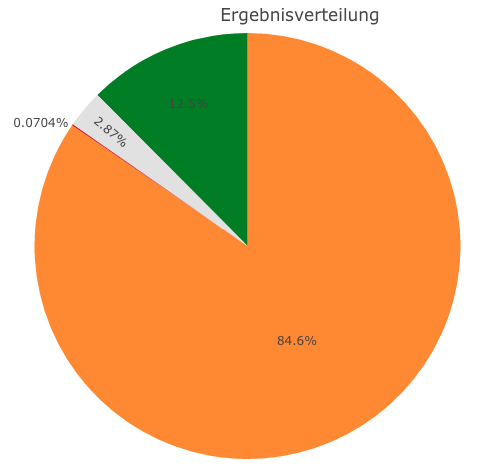
\includegraphics[width=5cm]{images/stats/diacertificate}
  \caption{Überprüfung des SSL-Zertifikats - Testergebnisverteilung}
  \label{fig:diacertificate}
\end{figure}
\todo{Samuel}

\subsection{Erkennung von Phishing}
\begin{figure}[H]
  \centering
  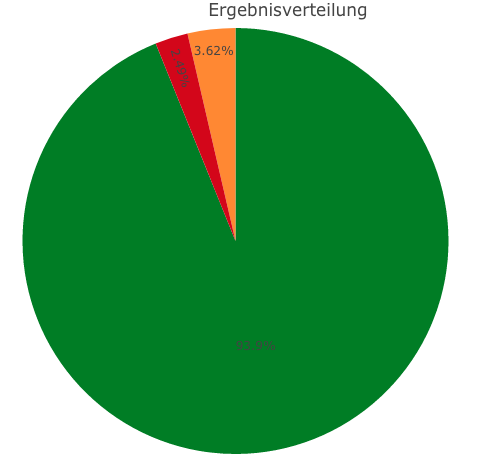
\includegraphics[width=5cm]{images/stats/diaphishing}
  \caption{Erkennung von Phishing - Testergebnisverteilung}
  \label{fig:diaphishing}
\end{figure}
\todo{Samuel}

\section{Bewertung der Ergebnisse}
